\subsection{E-step versus sleep phase}
\label{sec:estep_sleep_compare}

In this subsection, we compare the posteriors obtained by optimizing the sleep-phase objective~\eqref{eq:sleep_phase_summary} 
versus optimizing the E-step objective~\eqref{eq:e_step}, also known as the ELBO. 
We demonstrate on a toy example that there exist shallow optima in ELBO. In this example, the sleep phase objective is able to avoid the shallow optima, and the variational posterior is concentrated on the correct number of stars. We use simulated data with known PSF and background for this example, so the wake-phase (M-step) is not needed. 

In this toy example, we simulate a $20\times20$ image with one band, shown in Figure~\ref{fig:toy_example}. Each star has the same flux. The image is divided into four $10\times 10$ tiles, which are the input to the neural network. 
\begin{figure}[!h]
    \centering
    \vspace{-1em}
    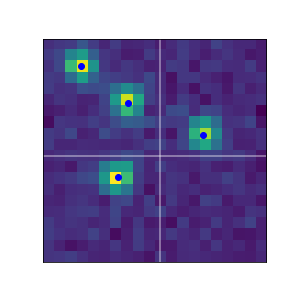
\includegraphics[width = 0.3\textwidth]{figures/vi_sleep_ex_figure.png}
    \vspace{-1.7em}
    \caption{The example $20\times 20$ image with four stars. The outlined $10\times 10$ tiles are inputs to the neural network. }
    \label{fig:toy_example}
\end{figure}

In our generative model, we set the Poisson prior parameter $\mu = 4$ and flux power law slope $\alpha = 0.5$. With these these prior parameters, we compare optimizing the ELBO and the sleep phase objective. First, in Figure~\ref{fig:optim_path} (top row), we evaluate the ELBO at the example $20\times 20$ image as the optimization proceeds. In the left-most plot, we optimized the ELBO using stochastic gradient descent with the REINFORCE estimator. The optimization did not converge, likely due to the high variance of the REINFORCE estimator. In the middle plot, we integrated out the discrete random variable, and computed stochastic gradients using the reparameterization trick. The resulting stochastic gradients exhibit lower variance, and the optimization was able to converge to stationary points. However, even with low-variance gradients, the variational distribution gets stuck at stationary points where the ELBO is non-optimal depending on the initialization (e.g. restarts 3 and 6). In contrast, optimizing the sleep phase consistently converges to a similar ELBO across all restarts. 

\begin{figure}[!ht]
    \centering
    \begin{subfigure}[t]{0.9\textwidth}
    \centering
    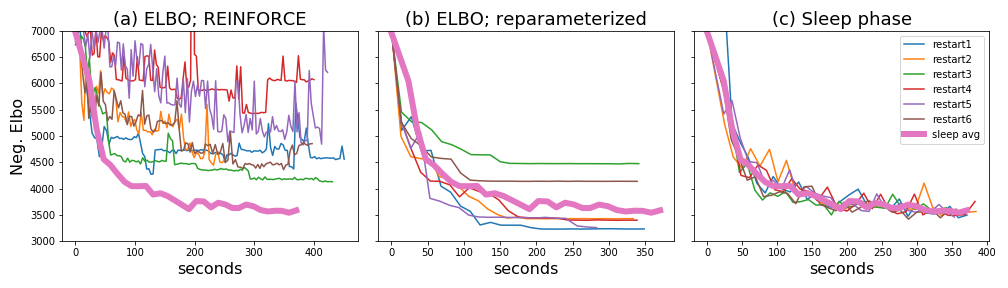
\includegraphics[width=\textwidth]{figures/optim_path_compare.png}
    \end{subfigure}
    
    \begin{subfigure}[t]{\textwidth}
    \centering
    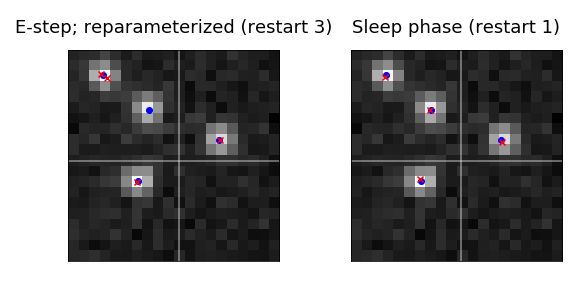
\includegraphics[width=0.4\textwidth]{figures/optim_path_detect_compare.png}
    \end{subfigure}
    \vspace{-3em}
    \caption{(Top) The ELBO as the optimization progresses, for six random restarts. Bold pink line is the sleep phase ELBO path, averaged over six restarts. (Bottom) Detections from two variational posteriors. Blue dots are true stars, red ``x" are MAP locations under the variational posterior. }
    \label{fig:optim_path}
\end{figure}

